\documentclass[font=default]{mpltx}
\usepackage{bm, ctex}
\usepackage{subfigure}
\usepackage{multirow}
% 以下至 \begin{document} 都仅是本文件为了方便额外定义的命令, 写报告时不需要.
\hypersetup{colorlinks=false}% 超链接带颜色
\usepackage{xcolor}
% 以上是本文件为了方便额外定义的命令, 写报告时不需要.
\linespread{1.5}
\begin{document}

\title{光泵磁共振} % 切合报告内容, 简短明确, 可以不同于讲义
\author{MaskedName} % 这里 \emailphone 一定要紧跟在 \author 后方
\emailphone{MyMail@stu.pku.edu.cn}{Tel}
% 如果改用 \email 则仅需要邮箱参数
\affiliation{北京大学物理学院\quad 学号: StudentID}
% % 可以使用 \zhdate 自动生成中文日期, 如
% \date{\zhdate{2020/12/1}}
% % 也可使用 babel 的 \localedate, 如
% \date{\localedate{2020}{12}{1}}
% % 两者均会输出 `2020 年 12 月 1 日'
% 下面的 \date 的参数是为了自动输出正确版本号, 正式报告请替换为上面的两种 \date 之一
\date{\zhdate{2023/10/25}}
\begin{abstract}
  光抽运是指通过特定的光使样品中的粒子数偏极化,使得粒子数分布不再服从玻耳兹曼分布的过程,这也是一种“偏极化”的过程。因为通过光抽运效应可以克服磁共振信号弱的特点,因此被广泛运用于研究原子的超精细结构和核磁共振上。本实验用铷灯的${\rm D_1\sigma^+}$作为抽运光,对铷样品的光抽运信号进行了观察。并且本实验通过光抽运效应和核磁共振的平衡测量铷原子的朗德$g$因子,还对地磁场的水平分量进行了简单的估测。本实验的结果和理论结果吻合得很好,证实了理论的正确性,也让我们对于理论和实验都有了更深的理解。
\end{abstract}
\keywords{光抽运效应,核磁共振,超精细结构}

\maketitle

\section{引言}
在磁场中,塞曼分裂导致的磁能级间距通常比较小,因此,产生磁共振现象所需的
能量通常位于射频或微波波段。此波段的电磁波能量要比光频段的能量小得多,普通的光谱仪器根本无法分辨,所以对于那些磁共振信号很微弱的样品(比如气体样品)很难探测。光泵,也称光抽运,是借助于光辐射获得原子基态超精细结构能级或塞曼子能级间粒子数的非热平衡分布的实验方法。在光泵磁共振技术中,一方面光抽运改变了磁能级上的粒子数分布,使更多的粒子参与磁共振,另一方面采取光探测的方法而不直接测量射频量子,从而克服了磁共振信号弱的缺点,把探测灵敏度提高了7\textasciitilde8个数量级。正因如此,光泵磁共振能够在弱磁场下(0.1\textasciitilde1 mT)精确检测气体原子能级的超精细结构。此外,若用激光把粒子激发到某一激发态,光泵磁共振也可用于研究原子能级的超精细结构。如今,光泵磁共振已广泛应用于基础物理研究,比如原子的磁矩、能级结构和$g$因子测量。此外,在量子频标、精确测量磁场等方面,这一方法也有很大的使用价值。

本实验研究铷原子的光泵磁共振现象,观察光抽运现象,并测量得到了铷原子的朗德$g$因子。
\section{理论\cite{book}}
\subsection{铷原子基态及最低激发态的能级}
天然铷中含量最大的同位素有两种:${\rm ^{85}Rb}$占72.15\%,${\rm ^{87}Rb}$占27.85\%。铷的基态是${\rm 5^2S_{1/2}}$,考虑精细结构,铷的最低激发态是${\rm 5^2P_{1/2}}$和${\rm 5^2P_{3/2}}$双重态。若进一步考虑原子核的自旋,那么核自旋与电子自旋及轨道角动量的耦合会使得能级进一步分裂,产生超精细结构。设原子核的自旋量子数为$I$,那么耦合的总角动量量子数为$F=I+J,\cdots,|I-J|$,其中$J$是电子自旋及轨道角动量耦合后的角动量量子数。

理论给出原子总角动量与总磁矩的关系为
\begin{equation}\label{mu_P_relation}
  \bm{\mu_F}=-g_F\frac{e}{2m}\bm{P_F},
\end{equation}其中
\begin{equation}\label{Lande_g}
  \begin{aligned}
    g_F&=g_J\frac{F(F+1)+J(J+1)-I(I+1)}{2F(F+1)},\\
    g_J&=1+\frac{J(J+1)-L(L+1)+S(S+1)}{2J(J+1)}.
  \end{aligned}
\end{equation}
${\rm ^{87}Rb}$的$I=3/2$,${\rm ^{85}Rb}$的$I=5/2$,利用\autoref{mu_P_relation}和\autoref{Lande_g},我们可以计算出这两种同位素在基态的朗德$g$因子:对于${\rm ^{87}Rb}$,在基态$F=2$的超精细结构能级上,其朗德因子为
\begin{equation}\label{Lande_g87}
  g_F({\rm ^{87}Rb},F=2)=\frac{1}{2}.
\end{equation}
对于${\rm ^{85}Rb}$,在基态$F=3$的超精细结构能级上,其朗德因子为
\begin{equation}\label{Lande_g85}
  g_F({\rm ^{87}Rb},F=3)=\frac{1}{3}.
\end{equation}

在外磁场下,这些超精细结构会导致可观测的能级分裂,即塞曼效应。磁量子数$m_F=F,F-1,\cdots,-F$,即能级分裂成$2F+1$个能量间隔基本相等的塞曼子能级。外磁场为$B_0$时,相邻塞曼子能级($\Delta m_F=\pm 1$)之间的能量差为
\begin{equation}
  \Delta E_{m_F}=g_F\mu_B B_0,
\end{equation}其中$\mu_B=\dfrac{e\hbar}{2m_e}$为玻尔磁子。
铷原子基态的塞曼子能级如\autoref{Rb_gndstate_Zeeman}所示。
\begin{figure}
  \centering
  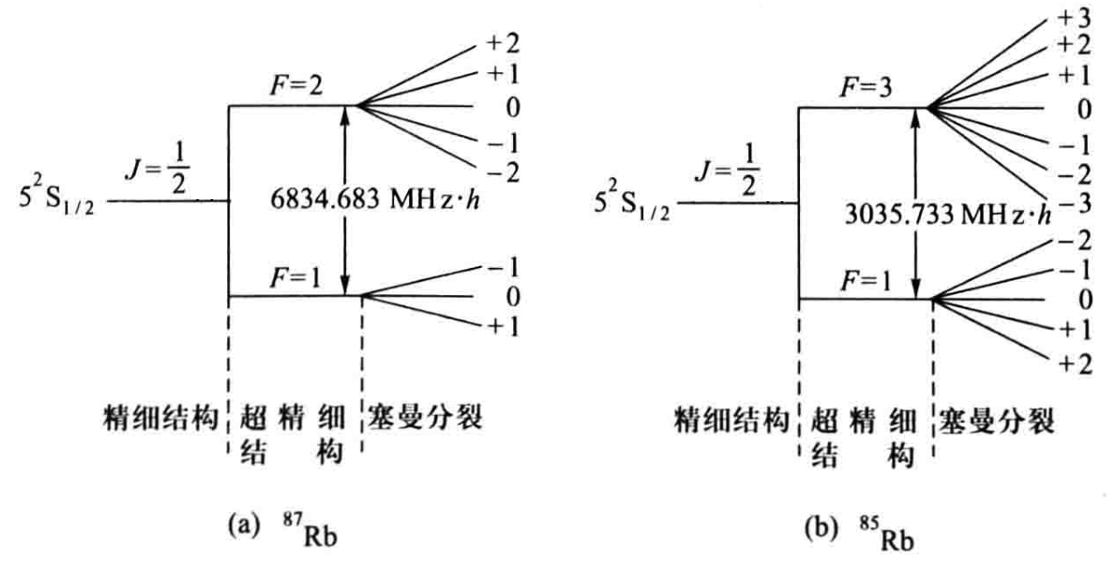
\includegraphics[width=0.8\linewidth]{fig/Rb_gndstate_Zeeman.png}
  \caption{\centering 铷原子基态塞曼能级示意图}
  \label{Rb_gndstate_Zeeman}
\end{figure}
\subsection{圆偏振光对铷原子的激发与光抽运效应}
假如我们能够用使得原子从${\rm 5^2S_{1/2}}$态跃迁到${\rm 5^2P_{1/2}}$态的左旋圆偏振光${\rm D_1\sigma^+}$作用在${\rm ^{87}Rb}$原子上,那么根据跃迁的选择定则,粒子就只能够跃迁到$\Delta m_F=+1$的态上。也就是说,基态$m_F=+2$的子能级上的粒子\textbf{不能跃迁}(因为${\rm 5^2P_{1/2}}$态没有$m_F=+3$的子能级)。然而,当原子从${\rm 5^2P_{1/2}}$能级跃迁回${\rm 5^2S_{1/2}}$能级的时候,粒子返回到基态各个子能级的概率是相等的(如\autoref{transition}所示)。这样,基态$m_F=+2$的子能级上的电子不能向上跃迁,但是可以接收跃迁回来的电子,经过若干循环之后,基态$m_F=+2$的子能级上的粒子数就会大大增加,即大量粒子被“抽运”到基态$m_F=+2$的子能级上,这就是光抽运效应。
\begin{figure}
  \centering
  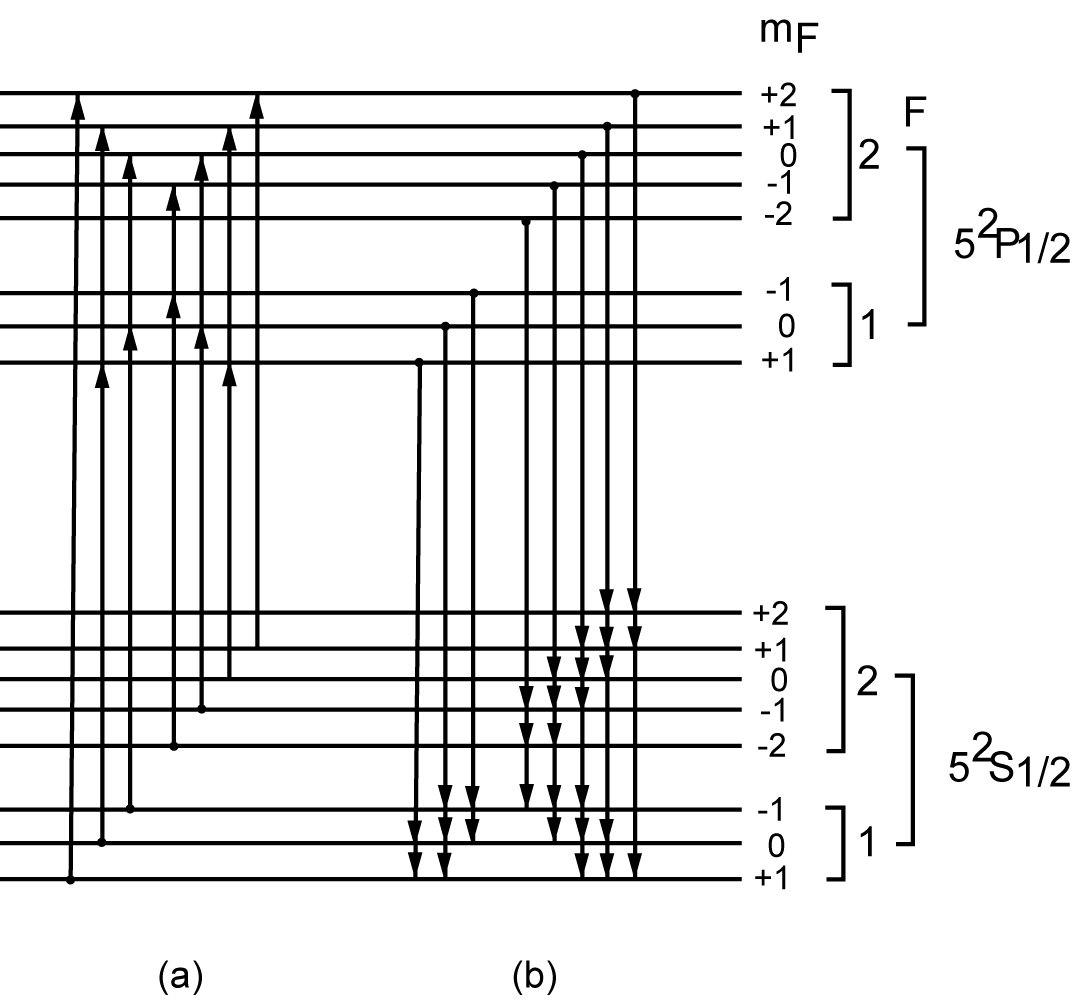
\includegraphics[width=0.6\linewidth]{fig/transition.png}
  \caption{(a) ${\rm ^{87}Rb}$基态粒子数吸收${\rm D_1\sigma^+}$的受激跃迁,基态$m_F=+2$的子能级上的电子不能向上跃迁;(b) ${\rm ^{87}Rb}$激发态粒子自发辐射回到基态各个子能级的概率是相等的。}
  \label{transition}
\end{figure}

光抽运效应各子能级上的粒子数偏离玻耳兹曼分布,也就是使粒子数分布在某一能级“偏极化”。有了这种偏极化,我们就可以在子能级之间的到较强的磁共振信号。

${\rm D_1\sigma^-}$同样可以实现光抽运,它将${\rm ^{87}Rb}$原子的大量粒子抽运到基态$m_F=-2$的子能级。值得注意的是,只有当入射光是圆偏振光的时候,光抽运效应才是最显著的。如果入射光是$\sigma^+$和$\sigma^-$混合的椭圆偏振光时,会因为没有办法使得基态$m_F=\pm2$中的一个子能级受激向上跃迁的概率为零而导致光抽运效应较圆偏振光小。如果入射光是$\pi$光,则不会发生光抽运效应。本实验正是通过调整光的偏振度以使光抽运效应最强来确保入射的光是圆偏振光的。
\subsection{弛豫过程}
在热平衡状态下,基态各子能级上的粒子数遵从玻尔兹曼分布。而光抽运可以使得能级之间的粒子数之差大大增加,使系统远远偏离热平衡分布状态。系统从非热平衡分布状态趋向于热平衡分布状态的过程叫做驰豫过程。在试验中为了保持原子分布的偏极化,我们必须要抑制驰豫过程。我们抑制驰豫过程的方法就是在样品中充进一定量的缓冲气体,以大大减少铷原子和器壁碰撞的机会。
\subsection{塞曼子能级之间的磁共振}
在垂直于恒定磁场$\bm{B_0}$的方向加一个频率为$\nu_1$的射频场$\bm{B_1}$,那么若满足共振条件
\begin{equation}\label{resonance_cond}
  h\nu_1=\Delta E_{m_F}=g_F\mu_B B_0,
\end{equation}
塞曼子能级之间将发生磁共振。对于${\rm ^{87}Rb}$原子,被抽运到基态$m_F=+2$子能级上的大量粒子,由于射频场$\bm{B_1}$的作用产生感应跃迁,即由$m_F=+2$跃迁到$m_F=+1$。同时由于抽运光的存在,处于基态$m_F\neq+2$子能级上的粒子又会被抽运到$m_F=+2$子能级上,感应跃迁和光抽运达到一个新的平衡。在发生磁共振的时候,$m_F\neq+2$子能级上的粒子大于不共振时,因此对于${\rm D_1\sigma^+}$光的吸收增大。由此我们可以通过观察透过样品的${\rm D_1\sigma^+}$光强的变化来判断是否达到磁共振。由于这种探测方式巧妙地将低频射频光子(1\textasciitilde10 MHz)的测量转换为光频光子($10^8$ MHz)的测量,因此可以使信号功率提高7\textasciitilde8个数量级。
\section{实验内容}
\subsection{实验装置\cite{manual}}
\subsubsection{概述}
本实验系统由主体单元、电源、辅助源、射频信号发生器及示波器五部分组成。见\autoref{experiment_setup}。
\begin{figure}[h]
  \centering
  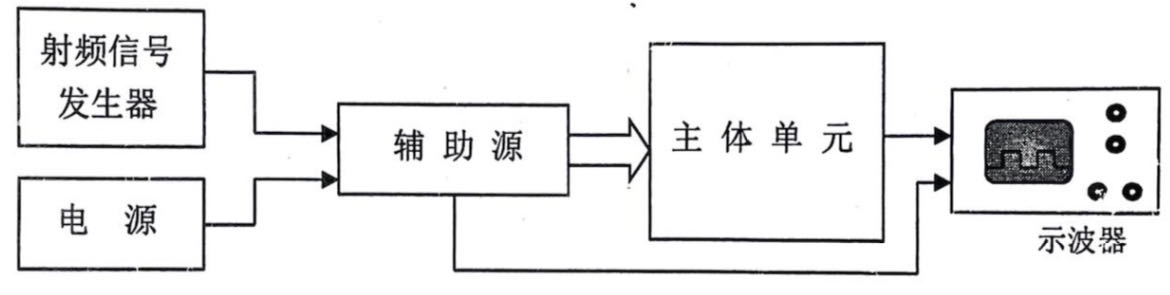
\includegraphics[width=0.6\linewidth]{fig/experiment_setup.jpg}
  \caption{光磁共振实验装置示意图}
  \label{experiment_setup}
\end{figure}
\subsubsection{主体单元}
主体单元是实验装置的核心,如\autoref{experiment_setup_main}所示。主体单元由高频无极放电铷灯、准直透镜、吸收池、聚光镜、光电探测器及亥姆霍兹线圈组成。

天然铷和惰性缓冲气体被充在直径约52 mm的玻璃泡内,两侧放着射频线圈,整体被放在圆柱形恒温槽内,称为“吸收池”。槽内温度约55 ${\rm ^\circ C}$左右。吸收池放置在两对亥姆霍兹线圈的中心。亥姆霍兹线圈能够产生水平直流磁场、竖直直流磁场和扫描磁场。光路上的两个透镜能够使铷灯发出的光平行通过吸收池,然后再汇聚到光电池上。干涉滤光镜从铷光谱中选出794.8 nm的光。偏振片和1/4波片使铷灯发出的光成为左旋圆偏振光。光电探测器能够接收投射光强度的变化,并把光信号转换为电信号。
\begin{figure}
  \centering
  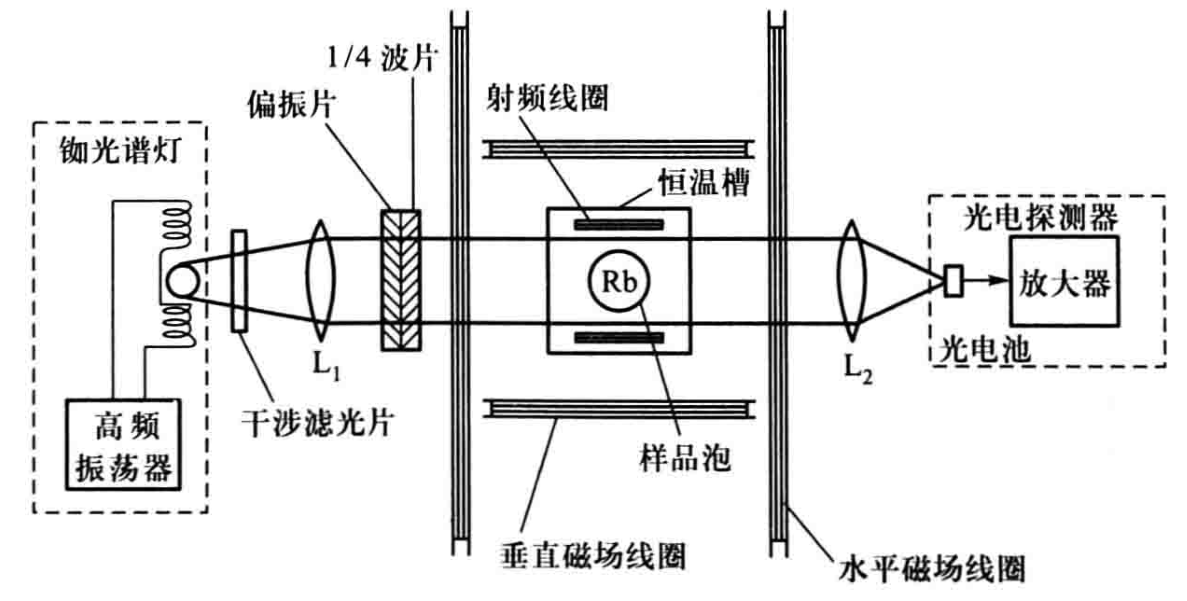
\includegraphics[width=0.7\linewidth]{fig/experiment_setup_main.png}
  \caption{光磁共振实验装置主体单元示意图}
  \label{experiment_setup_main}
\end{figure}
\subsubsection{辅助源}
辅助源为主体单元提供三角波、方波扫场信号及温度控制电路等,并设有“外接扫描”插座,可接SBR-1型示波器的扫描输出。
\subsubsection{射频信号发生器}
本实验装置中的射频信号发生器频率范围为100 kHz\textasciitilde1 MHz。射频信号发生器是为吸收池中的小射频线圈提供射频电流,使其产生射频磁场,激发铷原子产生共振跃迁。
\subsection{实验过程}
\subsubsection{装置的启动和调整}
启动装置。加热样品泡,使其温度在40 ${\rm ^\circ C}$\textasciitilde60 ${\rm ^\circ C}$之间并控温。加热铷灯,当铷灯泡的温度达到90 ${\rm ^\circ C}$左右开始控温(按下开关约30分钟后可达到目标温度)。随后,调节${\rm L_1}$、${\rm L_2}$的位置,使得射到光电接收器的总光量最大(这可以通过示波器上的光电接收器的信号确定)。

添加方波的扫描磁场,调大扫场幅度。预置垂直场电流为0.07 A左右用来抵消地磁场垂直分量。调节垂直场大小和偏振片的方向,使得光抽运信号幅度最大。根据我们在理论部分的讨论,当射到光电接收器的总光量最大时,就可以认为射在样品泡的光是圆偏振光。
\subsubsection{朗德$g$因子的测量}
扫场方式选择“三角波”(注意扫场幅度不能太大,否则会导致后面不同共振峰一起出现难以观察)。在不同的射频场频率下调节$B_0$的大小(或者在不同$B_0$大小时调节射频场的频率大小),先后找到${\rm ^{87}Rb}$和${\rm ^{85}Rb}$的共振信号,并记录此时$B_0$的大小(或者频率的大小)。

加上水平恒定场$B_0$和扫场$B_{\mbox{\zihao{7}扫}}$后,水平方向总磁场为
\begin{equation}
  B_{\parallel}=B_0+B_{{\mbox{\zihao{7}地}}\parallel}+B_{\mbox{\zihao{7}扫}}
\end{equation}其中$B_{{\mbox{\zihao{7}地}}\parallel}$为地磁场的水平分量。水平恒定场$B_0$可由下式算出
\begin{equation}\label{horizontal_mag}
  B_0=\frac{16\pi Ni}{5^{3/2}r}\times 10^{-3}\ Gs.
\end{equation}其中$N$是亥姆霍兹线圈的单边匝数,本实验中产生水平恒定场的亥姆霍兹线圈$N=250$,$r$为线圈的平均半径,本实验中产生水平恒定场的线圈$r=0.2387$ m,$i$为总电流。因此$B_0$可以算出,而$B_{{\mbox{\zihao{7}地}}\parallel}$和$B_{\mbox{\zihao{7}扫}}$的数值事先不知道,本实验使用两种方法来消除$B_{{\mbox{\zihao{7}地}}\parallel}$和$B_{\mbox{\zihao{7}扫}}$的影响。
\begin{enumerate}
  \item 测量共振频率和水平磁场的线性关系,通过斜率计算朗德$g$因子。
  \item 利用水平场和扫场的方向和共振条件结合测量朗德$g$因子(即通过改变水平磁场的方向测量不同的频率值,将两个频率值取平均以排除扫场直流分量和地磁水平分量的影响,见\autoref{method1})。
  \begin{equation}\label{method1}
    \left\{\begin{aligned}
      \frac{h\nu_1}{g_F\mu_B}&=B_0+B_{{\mbox{\zihao{7}地}}\parallel}+B_{\mbox{\zihao{7}扫}}\\
      \frac{h\nu_2}{g_F\mu_B}&=B_0-B_{{\mbox{\zihao{7}地}}\parallel}-B_{\mbox{\zihao{7}扫}}
    \end{aligned}\right.\to \frac{h}{g_F\mu_B}\frac{\nu_1+\nu_2}{2}=B_0.
  \end{equation}
\end{enumerate}
\subsubsection{估测地磁场的水平分量}
同测量$g$因子的方法类似,通过同时改变水平场和扫场的方向,测量到不同的频率,从而算出地磁场水平分量所对应的频率,见\autoref{method2}。
\begin{equation}\label{method2}
  \left\{\begin{aligned}
    \frac{h\nu_1}{g_F\mu_B}&=B_0+B_{{\mbox{\zihao{7}地}}\parallel}+B_{\mbox{\zihao{7}扫}}\\
    \frac{h\nu_2}{g_F\mu_B}&=B_0-B_{{\mbox{\zihao{7}地}}\parallel}+B_{\mbox{\zihao{7}扫}}
  \end{aligned}\right.\to \frac{h}{g_F\mu_B}\frac{\nu_1-\nu_2}{2}=B_{{\mbox{\zihao{7}地}}\parallel}.
\end{equation}
\section{实验结果与分析}
\subsection{光抽运过程的观察}
启动装置后,扫场方式选择“方波”,经过调节后,得到光抽运信号如\autoref{pump_light}所示。由于实际的弛豫时间较长,所以在光抽运还没有完全平衡的时候信号的方向就改变了,也就是不会出现平段的线型。但是我们仍然可以通过波形估测光抽运的时间常数。光抽运信号的半高宽为$\Delta X=12.6$ ms,所以光抽运信号随时间变化函数和时间常数为
\begin{equation}
  \begin{aligned}
    U&=U_0\left(1-\left(\frac{1}{2}\right)^{t/\tau}\right),\\
    \tau&=12.6\ {\rm ms}.
  \end{aligned}
\end{equation}
\begin{figure}[h]
  \centering
  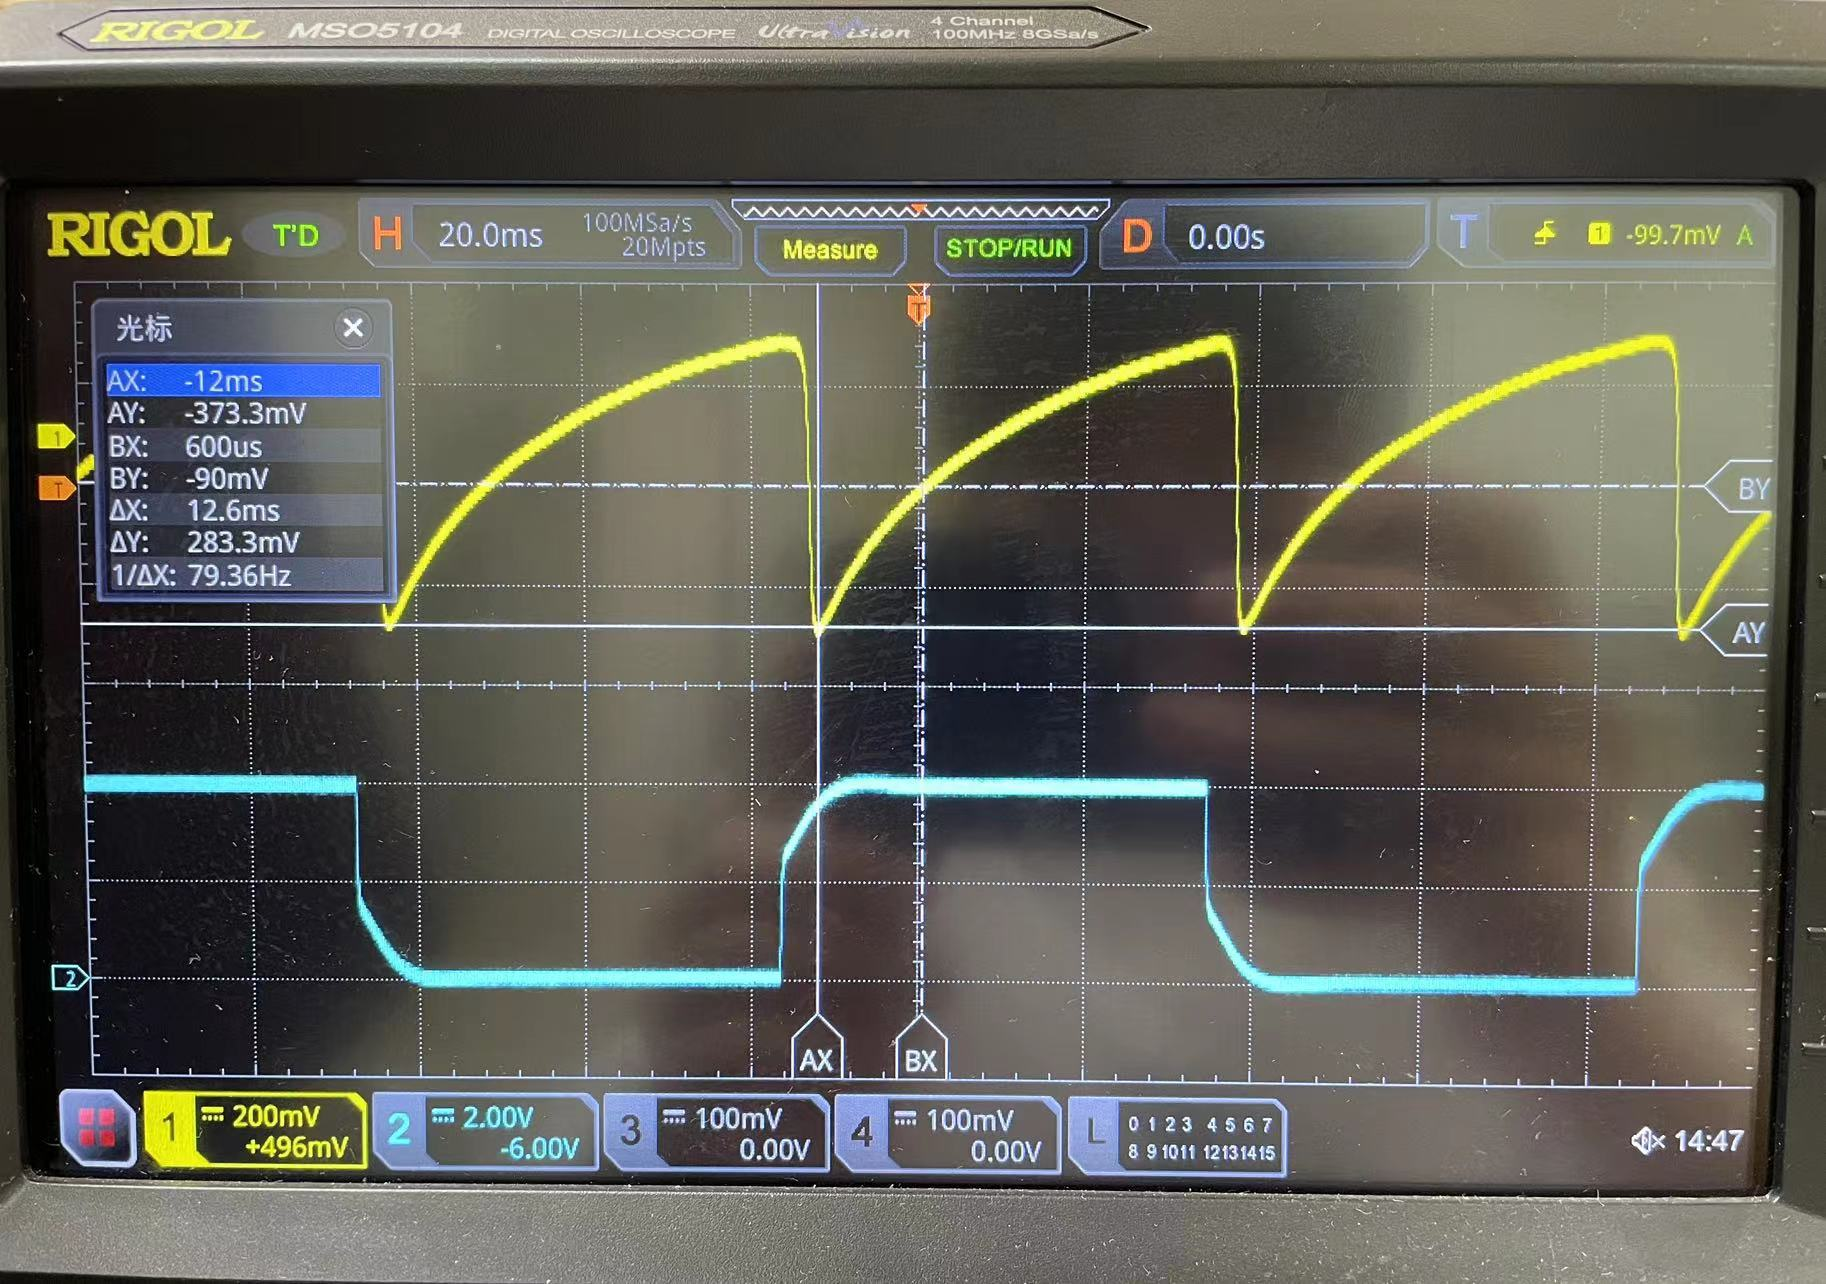
\includegraphics[width=0.5\linewidth]{fig/pump_light.jpg}
  \caption{光抽运信号}
  \label{pump_light}
\end{figure}
\subsection{由共振频率和水平磁场的线性关系测量朗德$g$因子}
在本实验中,我们通过调整射频频率和水平磁场的强度,观察${\rm ^{87}Rb}$和${\rm ^{85}Rb}$的磁共振信号。这些信号的出现位置对应了特定的磁共振跃迁。我们通过记录相应的电流信号$i$,然后对频率$\nu$和$i$的关系进行线性拟合来测量朗德$g$因子。

以50 kHz为间隔,将射频频率从800 kHz调节到1200 kHz,并在每个射频频率下调节水平场$B_0$的大小,分别找到${\rm ^{87}Rb}$和${\rm ^{85}Rb}$的共振信号(共振信号如\autoref{resonance_85_87} 所示,共振信号出现在三角波的波峰或者波谷,注意测量一种同位素时,要固定共振信号出现的位置),记录共振时的电流信号$i$,并对频率$\nu$和$i$做线性拟合,如\autoref{linfit}所示。

\begin{figure}[h]
  \centering 
  \subfigure[${\rm ^{87}Rb}$]{
  \label{resonance_87}
  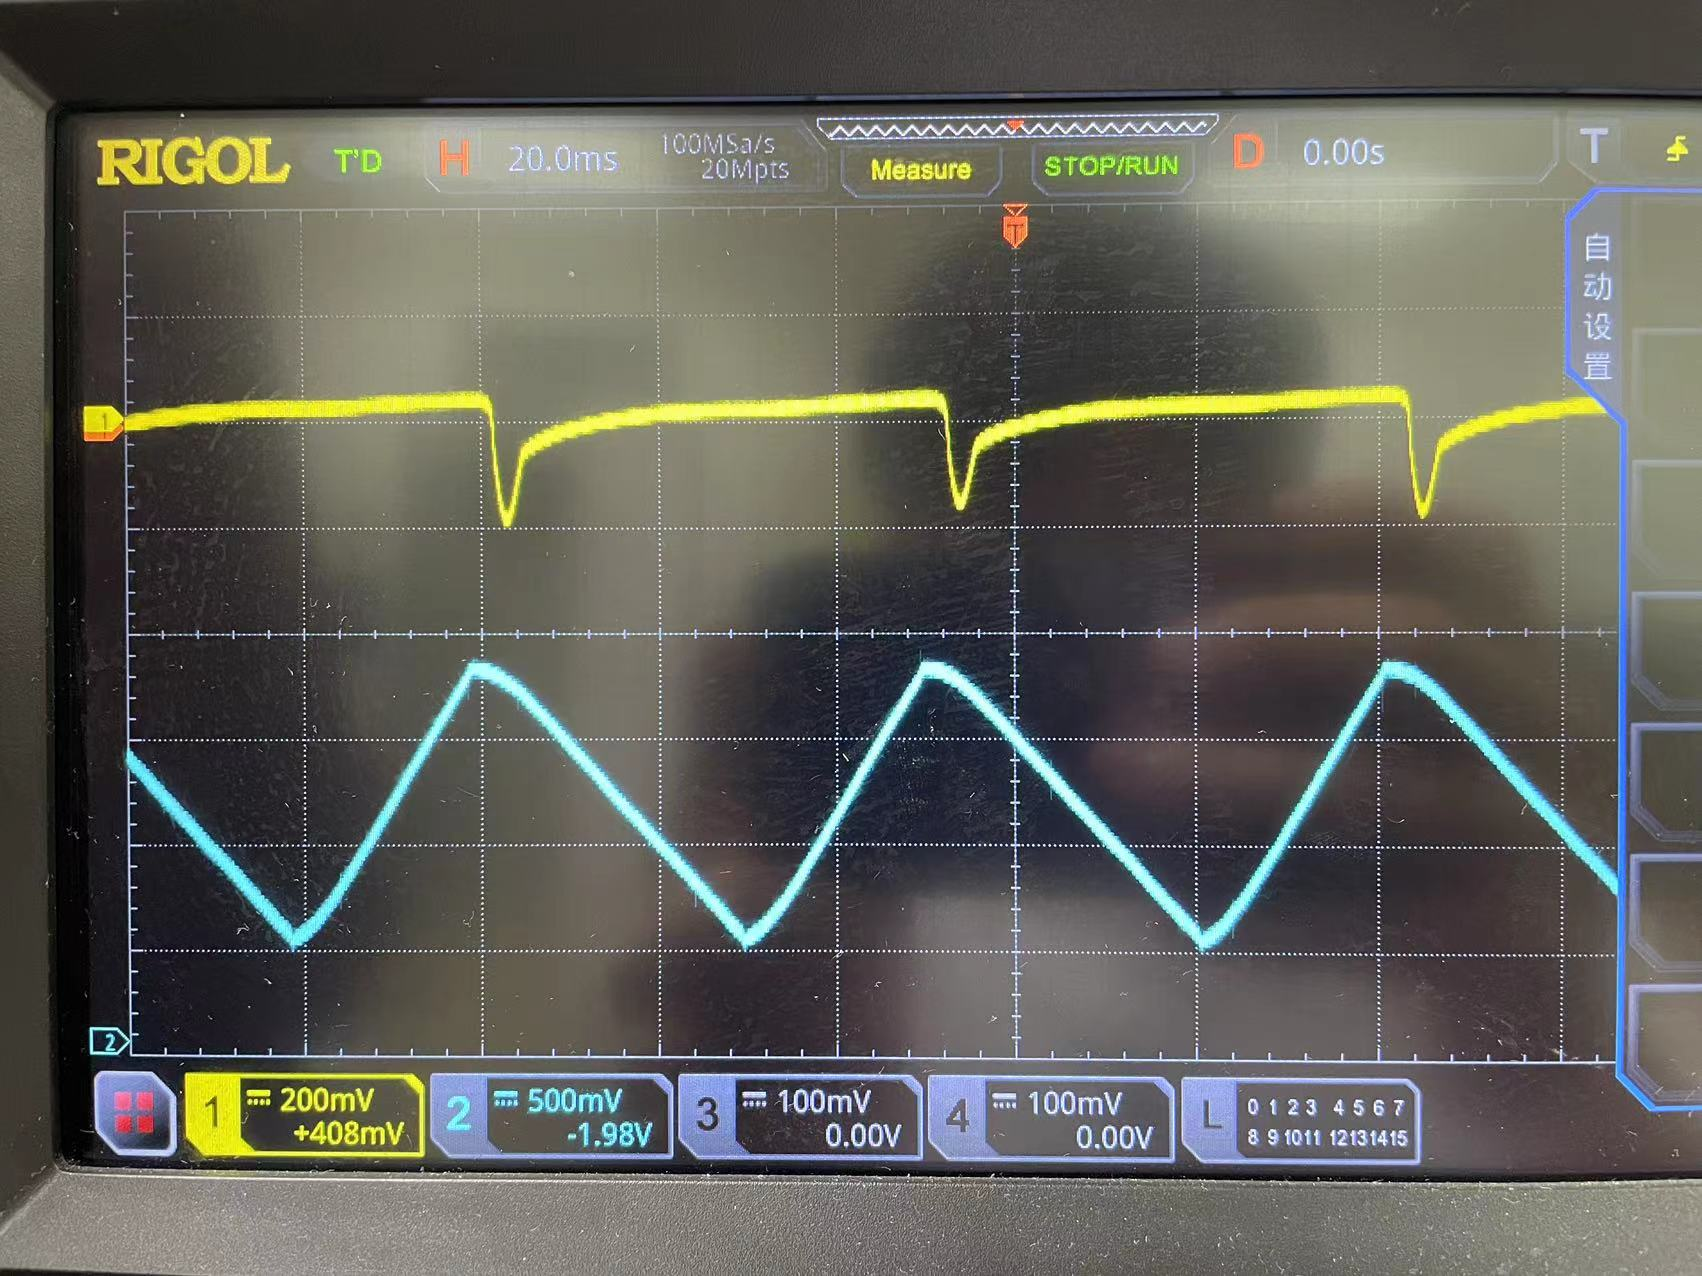
\includegraphics[width=0.4\linewidth]{fig/resonance_87.jpg}}\subfigure[${\rm ^{85}Rb}$]{
  \label{resonance_85}
  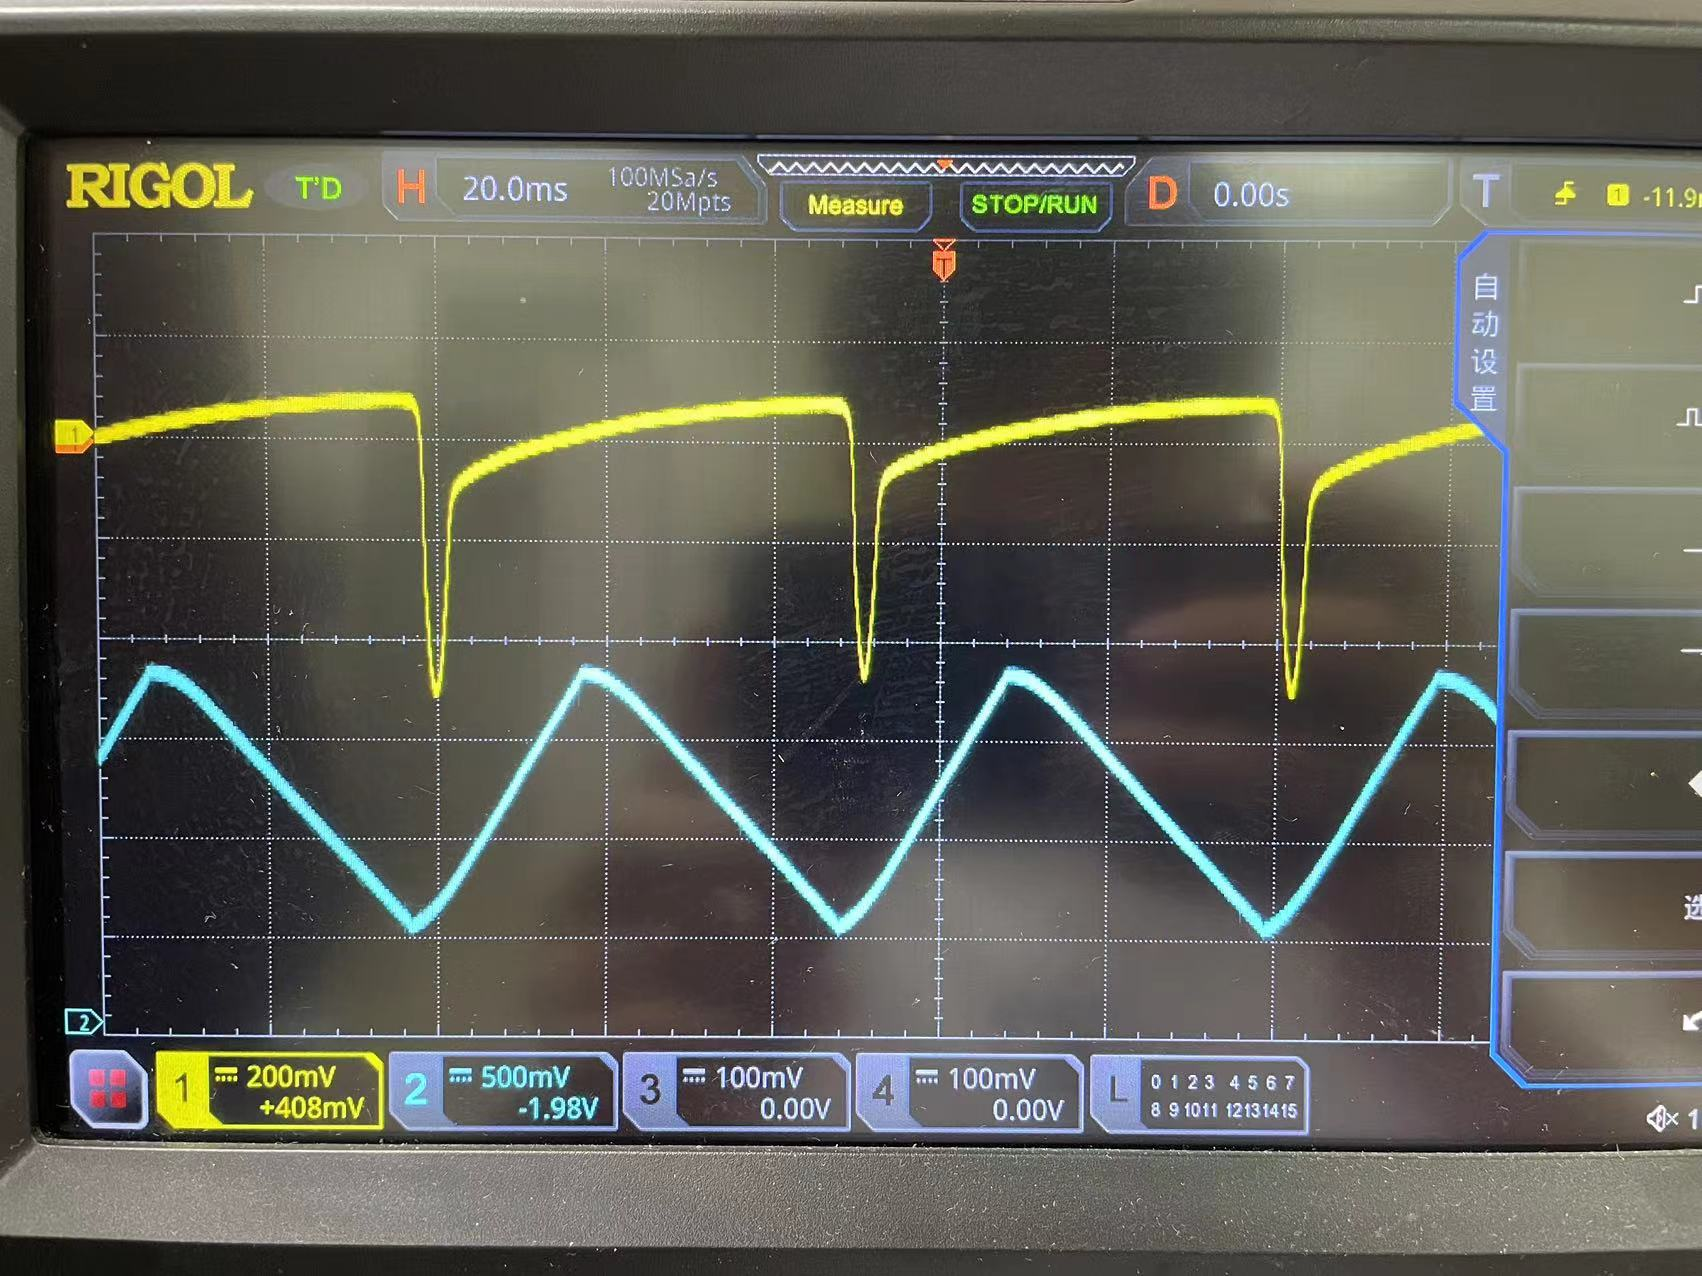
\includegraphics[width=0.4\linewidth]{fig/resonance_85.jpg}}
  \caption{${\rm ^{87}Rb}$和${\rm ^{85}Rb}$的共振信号。共振信号出现在三角波的波峰或者波谷。由于本实验使用的天然铷样本中${\rm ^{85}Rb}$占比更高,因此其在共振时吸收的${\rm D_1\sigma^+}$光也更多,共振峰更明显,据此我们可以分辨两种同位素的共振峰。}
  \label{resonance_85_87}
\end{figure}
\begin{figure}[h]
  \centering
  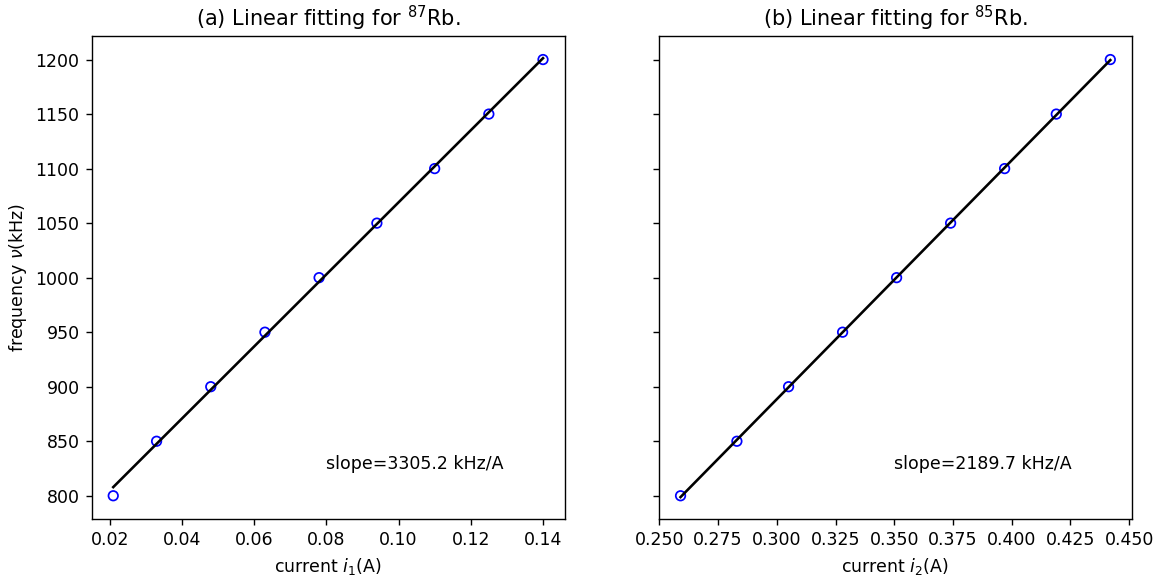
\includegraphics[width=0.9\linewidth]{fig/linfit.png}
  \caption{共振时的射频频率$\nu$和线圈电流$i$的线性拟合图\footnote{此图由Python的matplotlib.pyplot模块生成。}。(a) ${\rm ^{85}Rb}$的拟合直线,斜率为$k_1=3305.2$ kHz/A,相关系数$r$=0.9996;(b) ${\rm ^{87}Rb}$的拟合直线,斜率为$k_2=2189.7$ kHz/A,相关系数$r$=0.99998。}
  \label{linfit}
\end{figure}

根据\autoref{resonance_cond}和\autoref{horizontal_mag}可以得到共振时射频频率$\nu$和线圈电流$i$的线性关系(国际单位制下)
\begin{equation}
  \nu=\frac{g_F\mu_B}{h}\frac{16\pi N}{5^{3/2}r}\times 10^{-7}\cdot i.
\end{equation}
于是通过$\nu-i$图的斜率就可以求得朗德$g$因子的值。根据\autoref{linfit}的拟合结果,我们可以得到
\begin{equation}
  \begin{aligned}
    g_F(^{87}{\rm Rb},F=2)=0.5015,\\
    g_F(^{85}{\rm Rb},F=3)=0.3322.
  \end{aligned}
\end{equation}
我们将这些测量值与理论值进行比较,如\autoref{Lande_g87}和\autoref{Lande_g85}所示,相对误差分别为$\eta(^{87}{\rm Rb})=0.30\%$和$\eta(^{85}{\rm Rb})=0.33\%$。这说明我们的实验结果与理论值相当吻合,测量精度可以达到小数点后两位。

尽管实验结果令人满意,但仍然存在一些误差来源。首先,由于共振点的确定具有主观性,因此实际共振点可能存在一定的偏差。其次,由于地磁场的存在,它在水平面上的垂直分量可能会对实验测量产生一定的影响。最后,我们在调节竖直磁场的时候,由于我们是通过观察抽运信号大小调节竖直磁场的,而影响光抽运信号大小的因素有很多,所以事实上我们很难完全将地磁场的竖直分量的影响消去,这个残余下的竖直磁场会引入一定系统误差。

不过,尽管存在这些误差,我们的实验方法和测量结果都表明,光学磁共振实验是一种高度精确和非侵入性的技术,用于测量磁共振信号和朗德$g$因子,为磁共振研究提供了重要的工具和数据。在实验精度的提高方面,可以进一步改进共振点的准确定位和降低地磁场的影响,以实现更高的精度和准确性。
\subsection{利用水平场和扫场的方向和共振条件结合测量朗德$g$因子}
固定水平场和扫场大小,分别测量水平磁场正向和反向的共振射频频率,根据\autoref{method1}就可以计算朗德$g$因子。测量结果可以从\autoref{Landeg_measure}中得到:
\begin{equation}
  \begin{aligned}
    g_F(^{87}{\rm Rb},F=2)&=0.5010,\\
    g_F(^{85}{\rm Rb},F=3)&=0.3340.
  \end{aligned}
\end{equation}
\begin{table}[h]
  \caption{利用水平场和扫场的方向和共振条件结合测量朗德$g$因子的列表。本实验选择了三个线圈电流大小,并在不同电流大小下测量朗德$g$因子并求平均值。}
  \label{Landeg_measure}
  \begin{ruledtabular}
  \begin{tabular}{rrrrrrr}
    \multicolumn{1}{c}{$i$(A)} & \multicolumn{1}{c}{} & \multicolumn{1}{c}{$\nu_1$(kHz)} & \multicolumn{1}{c}{$\nu_2$(kHz)} & \multicolumn{1}{c}{$\overline{\nu}$(kHz)\footnote{$\overline{\nu}=\dfrac{\nu_1+\nu_2}{2}.$}} & \multicolumn{1}{c}{$g_F$} & \multicolumn{1}{c}{$\overline{g_F}$} \\\hline
    \multirow{2}*{0.401}                 & ${\rm ^{87}Rb}$                   & 1661.0                 & 986.0                  & 1323.5                & 0.5008                & 0.5010                \\
    ~  & ${\rm ^{85}Rb}$                   & 1108.0                 & 658.0                  & 883.0                 & 0.3341                & 0.3340                \\\hline
    \multirow{2}*{0.314}                 & ${\rm ^{87}Rb}$                   & 1376.0                 & 702.0                  & 1039.0                & 0.5021                &                       \\
    ~  & ${\rm ^{85}Rb}$                   & 917.0                  & 468.0                  & 692.5                 & 0.3346                &                       \\\hline
    \multirow{2}*{0.501}                 & ${\rm ^{87}Rb}$                   & 1988.0                 & 1314.0                 & 1651.0                & 0.5000                &                       \\
    ~  & ${\rm ^{85}Rb}$                   & 1326.0                 & 875.0                  & 1100.5                & 0.3333                &                      
  \end{tabular}
  \end{ruledtabular}
\end{table}将此测量结果和理论值进行比较和理论值进行比较,相对误差分别为$\eta(^{87}{\rm Rb})=0.20\%$和$\eta(^{85}{\rm Rb})=0.21\%$,说明实验值和理论值是基本吻合的。对比上一个方法,在这个方法中,我们固定水平场大小调节频率,而射频场频率的调节精度是要比水平场大小调节精度高的,所以这个方法测量出来的$g$因子值的误差也会相对小一些。对这个方法的误差分析基本同第一个方法,这里不再赘述。
\subsection{地磁水平分量的测量}
固定水平场和扫场大小,分别测量水平场和扫场同时正向和反向的共振射频频率,根据\autoref{method2}就可以计算地磁场水平分量。测量结果如\autoref{geomag_measure} 所示。
\begin{table}[h]
  \caption{地磁水平分量的测量列表。测量使用的是${\rm ^{85}Rb}$共振峰,朗德因子取$g_F=1/3$。}
  \label{geomag_measure}
  \begin{ruledtabular}
  \begin{tabular}{rrrrrr}
  \multicolumn{1}{c}{$i$(A)} & \multicolumn{1}{c}{$\nu_1$(kHz)} & \multicolumn{1}{c}{$\nu_2$(kHz)} & \multicolumn{1}{c}{$\Delta\nu$(kHz)\footnote{$\Delta\nu=\nu_1-\nu_2.$}} & \multicolumn{1}{c}{$\overline{\Delta\nu}$(kHz)} & \multicolumn{1}{c}{$\overline{B_{{\mbox{\zihao{7}地}}\parallel}}$(T)} \\\hline
  0.325  & 940.0    & 748.0   & 192.0    & 191.71   & 2.0546$\times 10^{-5}$ \\
  0.429    & 1169.0     & 978.0     & 191.0   &   &     \\
  0.483   & 1287.0   & 1095.0   & 192.0  &    &      \\
  0.535  & 1401.0    & 1208.0    & 193.0   &      &    \\
  0.596   & 1534.0     & 1342.0  & 192.0     &       &     \\
  0.645  & 1642.0    & 1451.0   & 191.0     &     &    \\
  0.389   & 1080.0    & 889.0    & 191.0   &     &                     
  \end{tabular}
  \end{ruledtabular}
\end{table}

测量得到地磁场的水平分量为
\begin{equation}
  B_{{\mbox{\zihao{7}地}}\parallel}=2.0546\times 10^{-5}\ {\rm T}.
\end{equation}在竖直方向上,竖直场线圈电流为$i=0.068$ A,因此我们也可以得到地磁场的竖直分量
\begin{equation}
  B_{{\mbox{\zihao{7}地}}\perp}=\frac{16\pi Ni}{5^{3/2}r}\times 10^{-7}=2.00\times 10^{-5}\ {\rm T}.
\end{equation}这里$N=100$,$r=0.1530$ m。总的地磁场大小为
\begin{equation}
  B_{\mbox{\zihao{7}地}}=\sqrt{B_{{\mbox{\zihao{7}地}}\parallel}^2+B_{{\mbox{\zihao{7}地}}\perp}^2}=2.87\times 10^{-5}\ {\rm T}.
\end{equation}
\section{结论}
本实验我们通过光抽运效应观察铷原子的核磁共振。光抽运的方法能够改变磁能级上的粒子分布,使得更多粒子参与磁共振。同时,这种测量透射光的方法巧妙地将低频射频光子的测量转换为光频光子的测量,使得测量到的信号功率大大提高。本报告给出了对光抽运信号的分析,使用了两种方法测量${\rm ^{87}Rb}$和${\rm ^{85}Rb}$的朗德$g$因子,并且最后对地磁场的水平分量进行了估测。本报告将实验值和理论值进行了比较,并进行了简单的误差分析,通过分析,也拓展了我们对这一现象和实验技术的认识。
\begin{acknowledgments}
  特别感谢薛建明老师在实验过程中的耐心指导和解答疑惑,他的指导使得整个实验过程更加顺利。同时,也要感谢\LaTeX 排版系统,它在整个报告的排版过程中发挥了重要作用,为我的报告提供了便捷和高效的排版解决方案。
\end{acknowledgments}

% bibliography 的参数是你的 *.bib 文件去掉后缀名后的部分

\begin{thebibliography}{}

  \bibitem{book} 吴思诚,荀坤。近代物理实验(第四版)(北京: 高等教育出版社,2015)
  \bibitem{manual} DH807A型光磁共振实验装置用户手册(北京大华无线电仪器有限责任公司)
\end{thebibliography}
  
\clearpage % 附录前另起一页
\appendix % 附录开始
\section{思考题}
\subsection{在如图的实验装置中为什么要用垂直磁场线圈抵消地磁场的垂直分量?不抵消会有什么不良后果?为什么}
如果存在较大的垂直磁场,那么加在样品上的总磁场$B_{tot}=\sqrt{B_\parallel^2+B_\perp^2}$始终不会等于零,这会导致粒子的塞曼子能级始终不会发生简并以及重新反向分裂的过程,而只会出现子能级间距的周期缩小和放大,因此我们就不能够观察到光抽运的弛豫过程。同时不为零的垂直磁场在我们测量朗德$g$因子时也会引入较大系统误差。
\subsection{本实验所用的射频场频率为$10^6$ Hz数量级,样品泡的温度约为$50\ {^\circ C}$,如果不考虑弛豫的后果,试估算利用光抽运探测磁共振比直接探测磁能级之间的磁共振跃迁的信号灵敏度提高了多少倍。}
磁共振跃迁放出的光子能量和射频场的频率一样,为$10^6$ Hz数量级(因为只考虑能量相对大小,这里我们取普朗克常数为1)。而利用光抽运探测磁共振跃迁,由于我们测量的是铷灯发出的${\rm D_1\sigma^+}$光,这个是可见光,因此光子能量的数量级为$10^14$ Hz。探测信号的灵敏度应该和光子的能量成正比,因此可以知道使用光抽运效应探测磁共振跃迁比直接探测跃迁信号的信号灵敏度提高了约$10^8$倍。

\section{实验记录本}
实验记录本。
\end{document}
